\documentclass[]{article}
\usepackage{amssymb,amsmath}
\usepackage{ifxetex,ifluatex}
\usepackage[english]{babel}
\ifxetex
  \usepackage{fontspec,xltxtra,xunicode}
  \defaultfontfeatures{Mapping=tex-text,Scale=MatchLowercase}
\else
  \ifluatex
    \usepackage{fontspec}
    \defaultfontfeatures{Mapping=tex-text,Scale=MatchLowercase}
  \else
    \usepackage[utf8]{inputenc}
  \fi
\fi
\usepackage{graphicx}
% We will generate all images so they have a width \maxwidth. This means
% that they will get their normal width if they fit onto the page, but
% are scaled down if they would overflow the margins.
\makeatletter
\def\maxwidth{\ifdim\Gin@nat@width>\linewidth\linewidth
\else\Gin@nat@width\fi}
\makeatother
\let\Oldincludegraphics\includegraphics
\renewcommand{\includegraphics}[1]{\Oldincludegraphics[width=\maxwidth]{#1}}
\ifxetex
  \usepackage[setpagesize=false, % page size defined by xetex
              unicode=false, % unicode breaks when used with xetex
              xetex,
              colorlinks=true,
              linkcolor=black]{hyperref}
\else
  \usepackage[unicode=true,
              colorlinks=true,
              linkcolor=black]{hyperref}
\fi
\hypersetup{breaklinks=true, pdfborder={0 0 0}}
\setlength{\parindent}{0pt}
\setlength{\parskip}{6pt plus 2pt minus 1pt}
\setlength{\emergencystretch}{3em}  % prevent overfull lines
%\setcounter{secnumdepth}{0}

\begin{document}

\begin{titlepage}
\centering \parindent=0pt
\newcommand{\HRule}{\rule{\textwidth}{1mm}}
\vspace*{\stretch{1}} \HRule\\[1cm]\Huge\bfseries
Homographies\\[0.7cm]
\large SIGB Assignment 2\\[1cm]
\HRule\\[4cm]  
Christoffer Stougaard Pedersen, Morten Roed Frederiksen, Sigurt
Bladt Dinesen


\small \{mrof,sidi,cstp\}\@itu.dk
\vspace*{\stretch{2}} \normalsize %
\begin{flushleft}
IT-University of Copenhagen \\
SIGB, F2013\\
Dan Witzner Hansen \& Diako Mardanbeigi \\
\today \end{flushleft}
\end{titlepage}

\tableofcontents
\pagebreak
\section{Introduction}

This is the second mandatory assignment for the course SIGB F2013. In this
assignment we will explore the use of homographies in order to transform points
between
planes in images, texture mapping, and camera calibration. This will
be done in the programming language python with help from the libraries
opencv,numpy, and matplotlib.


\section{Augmented reality}

What we want to achieve:
We want to calibrate a camera using cv2 implemented methods.
Grab images of the calibration chessboard.
Project a box onto the images, with a camera class calculated for each
image. 

\subsection{Camera Calibration}

Why do we calibrate?
We want to be aware of the factors within the camera, that may affect the
displaying of our  image.

\textbf{The focal length}, a measure for how much the used lens
centers/bends the light

\begin{figure}[!htbp]
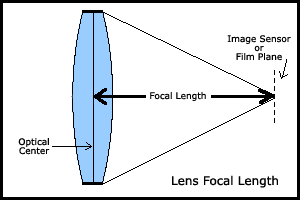
\includegraphics{pics/focal_length.png}
\caption{Focal length}
\label{fig:focal_length}
\end{figure}

\textbf{The image center} (according to the camera), this is not always just
positioned at precisely at half the height, half the width.
\textbf{Scaling factors}. Scaling can occur both horizontally and vertically. 
\textbf{Skew factors}.  Skewing may happen.
\textbf{Lens distortion}.  Cheap lenses may produce pin/cushion effects, and some
cameras may even add additional lenses to correct these issues.

All these factors needs to be taken into consideration when we wish to
calculate projections from the world coordinates to image coordinates. 

We calibrate the camera by using the cv2 implementation and a standard
calibration chessboard pattern. 


\subsection{Camera internal matrixes}

The camera consists of Intrinsic and extrinsic parameters,
K * [R | T]
The extrinsic parameters consists of a 3x3 rotation matrix (R )and a
translation vector (T). The translation vector expresses the origin of the world
coordinate system in camera coordinates. 
These transforms the coordinates from 3d world coordinates to 3d camera
coordinates. 

The intrinsic matrix (K) contains 5 parameters.

\begin{figure}[!htbp]
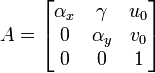
\includegraphics{pics/intristic_parameters.png}
\caption{Intrinsic/camera -matrix (here represented by "A")}
\label{fig:intrinsic_parameters}
\end{figure}

Alpha-X = focal length * scale factor(for x-coords), and 

Alpha-Y = focal length * scale factor(for y-coords). These converts real world
length (in mm) to pixel distance. 

$\gamma$  is the skew coefficient, and u0 v0 are the camera center.


\subsection{projecting and image using K* [I | O]}

\begin{figure}[H]
\centering
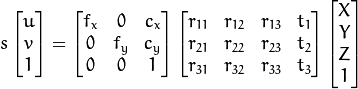
\includegraphics{pics/homogenious_projection.png}
\label{homogenious_projection}
\end{figure}

When we want to project 3d coordinates to the 2d image plane we multiply the
coord vector by K * [I | O] matrixes and converts the result to
homogeneous coords on the 2d image plane. Here (X,Y,Z) is the world
coordinate and (U,V) is the image coordinate. 
The column vectors [r1, r2, r3] of the “I” extrinsic matrix represent the
directions of the world-axes in camera coordinates.


\subsection{Theory of our implementation}

When we want to project a box onto different surfaces, we need to
calculate new camera parameters K * [I | O] each time we change
scene/angle. Some parameters can be reused. The intrinsic camera matrix “K”
doesn’t rely on anything from the scene and remains the same once calibrated. 

The first projection and the first camera.
The first camera initialized in our implementation uses the the fact that our
camera has been calibrated, and the projection plane is fully frontal and dead
center (in theory).
Therefore, no rotation and no translation in happening in the projection and
the [I | O] part of our camera class is equal to the identity matrix
(changes nothing when multiplied onto another matrix). 

The box cordinates are projected in the center of the image and viewed
directly from above.
As the projection is a perspective projection not a parallel projection, the
box appears realisticly to “pop” out from the surface. 

\begin{figure}[H]
\center
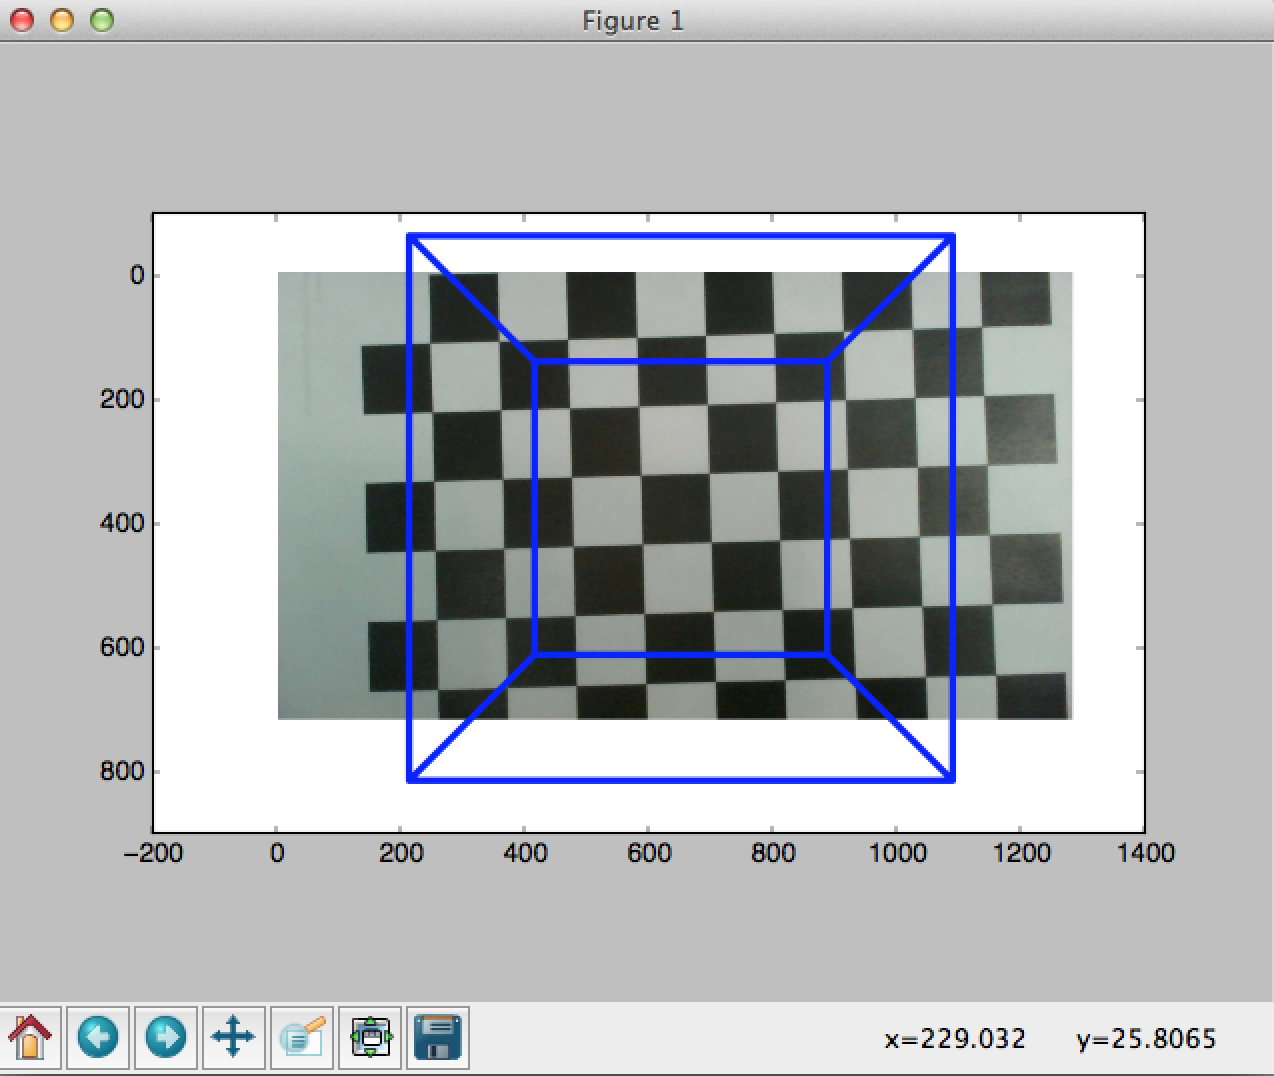
\includegraphics{pics/aug1}
\caption{The first projection onto a fully frontal surface.}
\label{aug1}
\end{figure}

When we want to project the box realistically onto the chessboard when the image
is no longer fully frontal, we calculate a new camera class.
This is done through the following steps:
1.We estimate a homography between the two chessboard surfaces, gaining a 2d
conversion between the two chessboards/scenes.
2.We multiply the existing camera with the homography as using the
homography is a perfectly valid way of projecting the 2D “X” and “Y” coords.
3.We estimate values for the “Z” axis by taking the cross product of the “X”
and “Y” axis-vectors. Thsi will always be orthogonal to both these
vectors, and therefore a good, but not precise estimation of the z-axis.


\begin{figure}[H]
\center
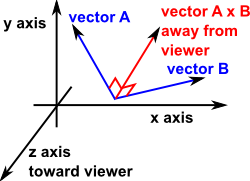
\includegraphics{pics/crossProduct.png}
\caption{Estimating the third axis from the existing two by taking the AxB crossproduct.}
\label{cross_product}
\end{figure}


\subsection{Our Code: (the important lines)}

\begin{verbatim}
//This line initializes the first camera, with K * [I | O] .

 cam1 = Camera(hstack((K,dot(K,array([[0],[0],[-1]])) )) )

//We estimate the homography “H” between the two chessboards by detecting 4 corners in each image.

H = estimateHomography(I1Corners, I2Corners)

//The homography is used on the existing (frontal) camera

  cam2 = Camera(dot(H,cam1.P))

//We isolate the [Rotation | translation] matrix by multiplying by inverse of “K” calibration matrix.

 A = dot(linalg.inv(K),cam2.P[:,:3]) 

//The intrinsic parameters are initialized. The X,Y axes are already valid after being multiplied by the homography matrix, and the third column vector is estimated with the cross product.

    A = array([A[:,0],A[:,1],np.cross(A[:,0],A[:,1],axis=0)]).T

// The calibration matrix is added again by multiplication, and the result is stored in the new camera.

    cam2.P[:,:3] = np.dot(K,A[0])

 //The box coordinates are projected onto the plane with the second camera

box_cam2 = np.array(cam2.project(toHomogenious(box)))
\end{verbatim}

Note: Concerning getting a better homography we found that using the
original pattern image “pattern.png” instead of our own frontal webcam
photo produced a better result. It proved hard to capture a frontal image
without any rotation or translation. At least with using the pattern image we
avoid rotations, but a translation is still present as the pattern is not
completely centered. 


\subsection{Augmentation, our results}

\begin{figure}[H]
\center
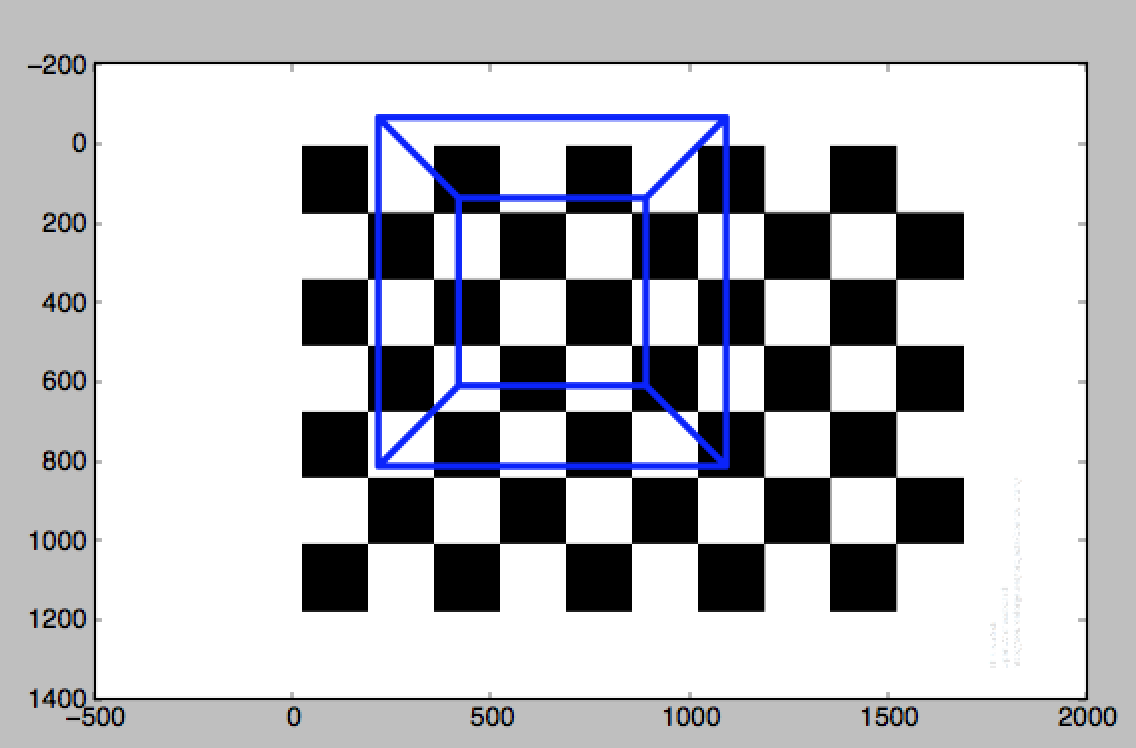
\includegraphics{pics/result0.png}
\caption{Our first projection onto the pattern image. The perspective projection effect is very visable on this image. Notice the translation of the pattern. This will affect the placement of the box on the rest of the images.}
\label{result0}
\end{figure}

\begin{figure}[H]
\center
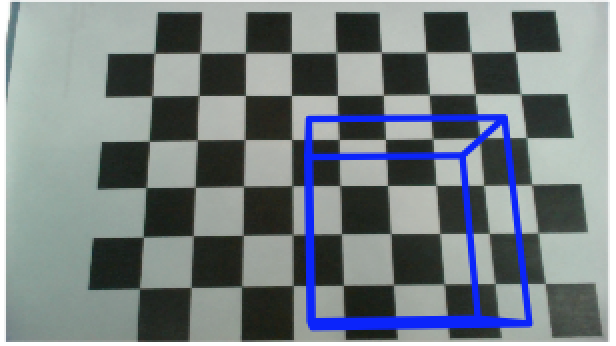
\includegraphics{pics/result1.png}
\caption{On this image the chessboard is only moved slightly away from the full frontal position. The position of the boc on the pattern doesn’t correspond to the position of the pattern image, but is consistent with the rest of the images.}
\label{result1}
\end{figure}

\begin{figure}[H]
\center
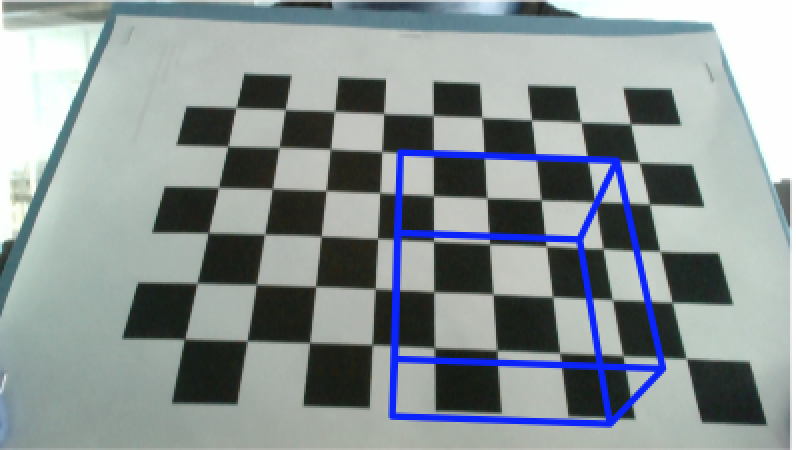
\includegraphics{pics/result2.png}
\caption{The 3d effect gets more pronounced as the chessboard is moved further away from the frontal position. The box doesn’t look completely even, but that is caused by the estimation of the z axis.}
\label{result2}
\end{figure}

\begin{figure}[H]
\center
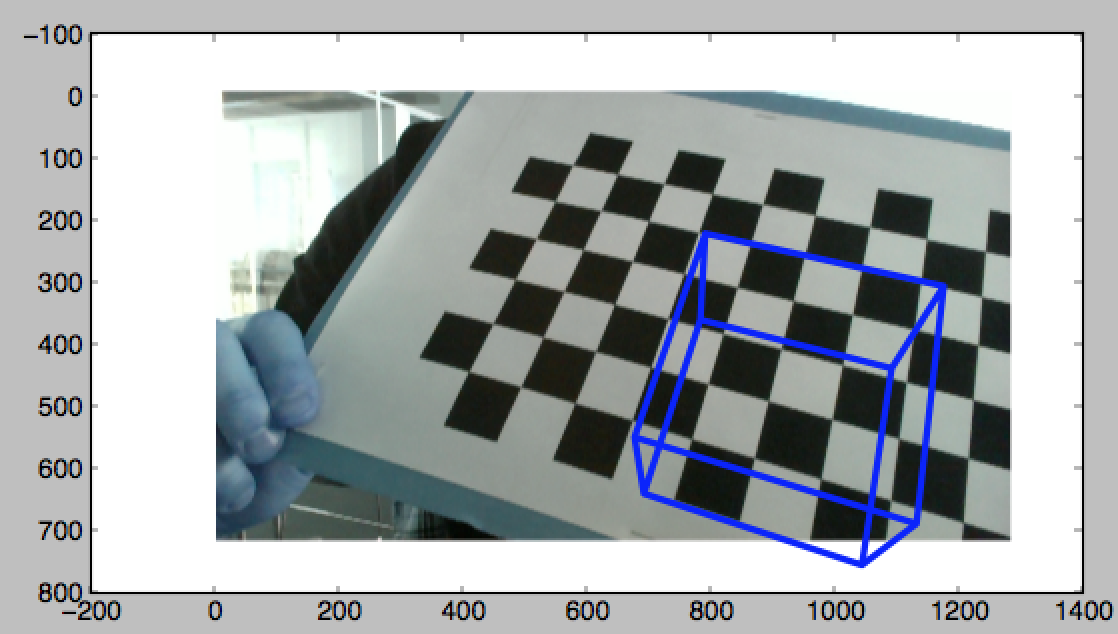
\includegraphics{pics/result3.png}
\caption{As we see here. The projection and plotting of the box, doesn’t care about image limits in this implementation. Gives a pretty nice effect though. (Best viewed with 3d glasses :-))}
\label{result3}
\end{figure}


\begin{figure}[H]
\center
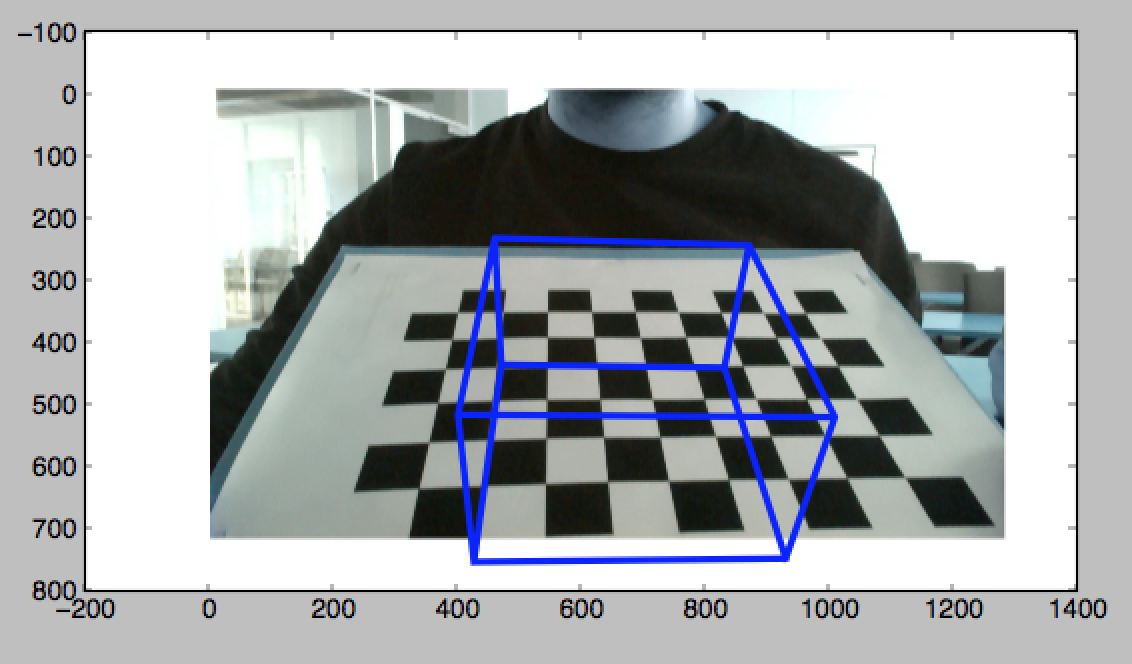
\includegraphics{pics/result4.png}
\caption{The augmentation effect works best when the surroundings are visible. Also note that the box looks a bit skewed/uneven but follows the chessboard pattern exactly because of the homography.}
\label{result4}
\end{figure}

\begin{figure}[H]
\center
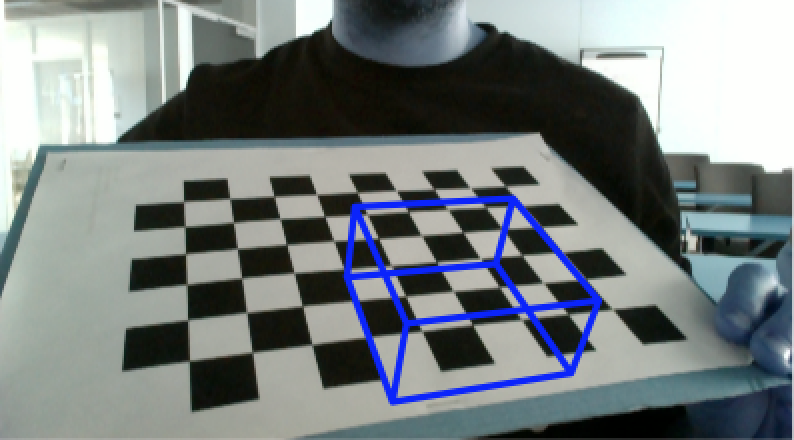
\includegraphics{pics/result5.png}
\caption{Last image. Lets just notice that it looks awesome. Next stop cool 3d models projected on family photos.}
\label{result5}
\end{figure}


\subsection{Taking it live}

As soon as the method for augmenting a box on a single frame is in place,
expanding to live view is a pretty easy task. 
In the old augmentation method we did a fair share of redundant
calculations. In order for the live augmentation to run smoothly, these had
to be moved out so they’ll only be done once.

Reading in the pattern image, converting it to greyscale and loading the
calibration-matrixes were moved out to global vars instead.

\begin{verbatim}
I1 = cv2.imread("pattern.png")
I1Gray = cv2.cvtColor(I1,cv2.COLOR_RGB2GRAY)
K, dist_coefs = calibrate.loadMatrixes()
\end{verbatim}

Calculating the corderns of the original pattern image, getting the box cords
and initialising the first camera instance also only needed to be done once.

\begin{verbatim}
I1Corners = getCornerCoords(I1Gray)
box = cube_points((0,0,0),0.3)
cam1 = Camera(hstack((K,dot(K,array([[0],[0],[-1]])) )) )
\end{verbatim}

Notice that these are only minor speed improvements, as each frame still has
some heavy calculations to be made:

\subsubsection{We still have to}
Find the chessboard corners on the supplied frame

\begin{verbatim}
I2Corners = getCornerCoords(I2Gray)
\end{verbatim}

Calculate a homography between the two chessboard 2d surfaces.

\begin{verbatim}
H = estimateHomography(I1Corners, I2Corners)
\end{verbatim}

Project the box cords onto the new surface.

\begin{verbatim}
box_cam2 = np.array(cam2.project(toHomogenious(box)))
\end{verbatim}

And then draw the box in the frame.
The end result could of course be improve further (as always), but for the scope
of this assignment we think the result is very acceptable, and undeniably cool
:-)
See. Aug.avi for the result video.



\section{Augmented reality}

What we want to achieve:
We want to calibrate a camera using cv2 implemented methods.
Grab images of the calibration chessboard.
Project a box onto the images, with a camera class calculated for each
image. 

\subsection{Camera Calibration}

Why do we calibrate?
We want to be aware of the factors within the camera, that may affect the
displaying of our  image.

\textbf{The focal length}, a measure for how much the used lens
centers/bends the light

\begin{figure}[!htbp]
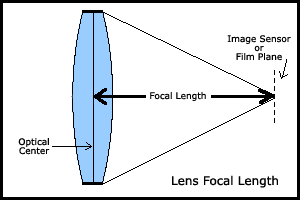
\includegraphics{pics/focal_length.png}
\caption{Focal length}
\label{fig:focal_length}
\end{figure}

\textbf{The image center} (according to the camera), this is not always just
positioned at precisely at half the height, half the width.
\textbf{Scaling factors}. Scaling can occur both horizontally and vertically. 
\textbf{Skew factors}.  Skewing may happen.
\textbf{Lens distortion}.  Cheap lenses may produce pin/cushion effects, and some
cameras may even add additional lenses to correct these issues.

All these factors needs to be taken into consideration when we wish to
calculate projections from the world coordinates to image coordinates. 

We calibrate the camera by using the cv2 implementation and a standard
calibration chessboard pattern. 


\subsection{Camera internal matrixes}

The camera consists of Intrinsic and extrinsic parameters,
K * [R | T]
The extrinsic parameters consists of a 3x3 rotation matrix (R )and a
translation vector (T). The translation vector expresses the origin of the world
coordinate system in camera coordinates. 
These transforms the coordinates from 3d world coordinates to 3d camera
coordinates. 

The intrinsic matrix (K) contains 5 parameters.

\begin{figure}[!htbp]
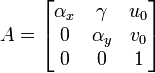
\includegraphics{pics/intristic_parameters.png}
\caption{Intrinsic/camera -matrix (here represented by "A")}
\label{fig:intrinsic_parameters}
\end{figure}

Alpha-X = focal length * scale factor(for x-coords), and 

Alpha-Y = focal length * scale factor(for y-coords). These converts real world
length (in mm) to pixel distance. 

$\gamma$  is the skew coefficient, and u0 v0 are the camera center.


\subsection{projecting and image using K* [I | O]}

\begin{figure}[H]
\centering
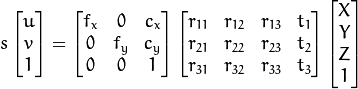
\includegraphics{pics/homogenious_projection.png}
\label{homogenious_projection}
\end{figure}

When we want to project 3d coordinates to the 2d image plane we multiply the
coord vector by K * [I | O] matrixes and converts the result to
homogeneous coords on the 2d image plane. Here (X,Y,Z) is the world
coordinate and (U,V) is the image coordinate. 
The column vectors [r1, r2, r3] of the “I” extrinsic matrix represent the
directions of the world-axes in camera coordinates.


\subsection{Theory of our implementation}

When we want to project a box onto different surfaces, we need to
calculate new camera parameters K * [I | O] each time we change
scene/angle. Some parameters can be reused. The intrinsic camera matrix “K”
doesn’t rely on anything from the scene and remains the same once calibrated. 

The first projection and the first camera.
The first camera initialized in our implementation uses the the fact that our
camera has been calibrated, and the projection plane is fully frontal and dead
center (in theory).
Therefore, no rotation and no translation in happening in the projection and
the [I | O] part of our camera class is equal to the identity matrix
(changes nothing when multiplied onto another matrix). 

The box cordinates are projected in the center of the image and viewed
directly from above.
As the projection is a perspective projection not a parallel projection, the
box appears realisticly to “pop” out from the surface. 

\begin{figure}[H]
\center
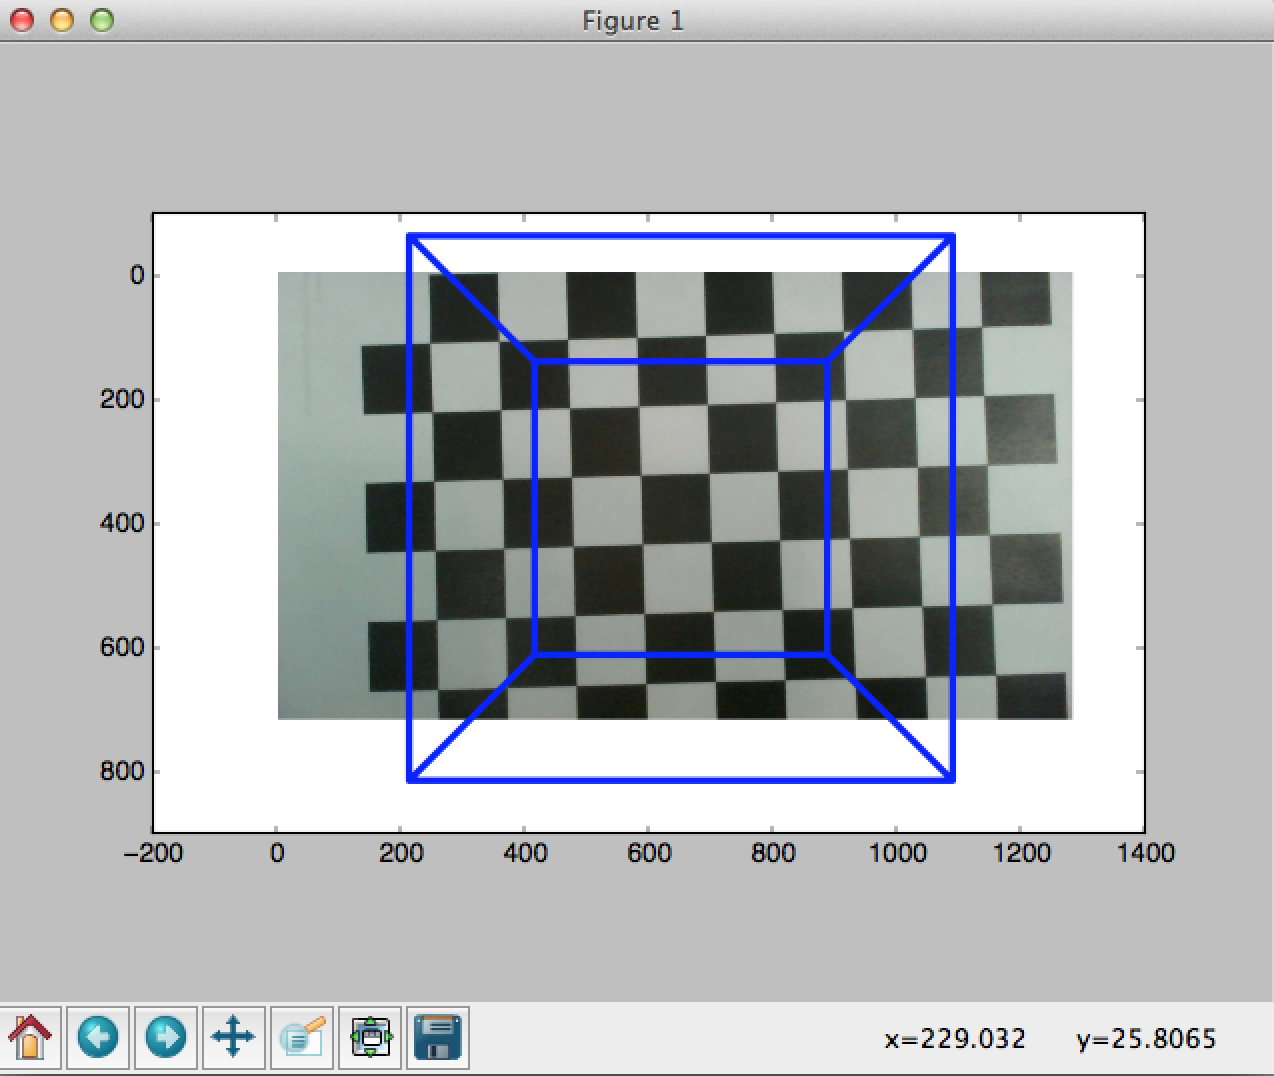
\includegraphics{pics/aug1}
\caption{The first projection onto a fully frontal surface.}
\label{aug1}
\end{figure}

When we want to project the box realistically onto the chessboard when the image
is no longer fully frontal, we calculate a new camera class.
This is done through the following steps:
1.We estimate a homography between the two chessboard surfaces, gaining a 2d
conversion between the two chessboards/scenes.
2.We multiply the existing camera with the homography as using the
homography is a perfectly valid way of projecting the 2D “X” and “Y” coords.
3.We estimate values for the “Z” axis by taking the cross product of the “X”
and “Y” axis-vectors. Thsi will always be orthogonal to both these
vectors, and therefore a good, but not precise estimation of the z-axis.


\begin{figure}[H]
\center
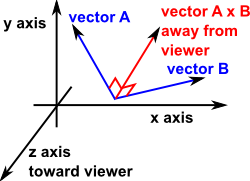
\includegraphics{pics/crossProduct.png}
\caption{Estimating the third axis from the existing two by taking the AxB crossproduct.}
\label{cross_product}
\end{figure}


\subsection{Our Code: (the important lines)}

\begin{verbatim}
//This line initializes the first camera, with K * [I | O] .

 cam1 = Camera(hstack((K,dot(K,array([[0],[0],[-1]])) )) )

//We estimate the homography “H” between the two chessboards by detecting 4 corners in each image.

H = estimateHomography(I1Corners, I2Corners)

//The homography is used on the existing (frontal) camera

  cam2 = Camera(dot(H,cam1.P))

//We isolate the [Rotation | translation] matrix by multiplying by inverse of “K” calibration matrix.

 A = dot(linalg.inv(K),cam2.P[:,:3]) 

//The intrinsic parameters are initialized. The X,Y axes are already valid after being multiplied by the homography matrix, and the third column vector is estimated with the cross product.

    A = array([A[:,0],A[:,1],np.cross(A[:,0],A[:,1],axis=0)]).T

// The calibration matrix is added again by multiplication, and the result is stored in the new camera.

    cam2.P[:,:3] = np.dot(K,A[0])

 //The box coordinates are projected onto the plane with the second camera

box_cam2 = np.array(cam2.project(toHomogenious(box)))
\end{verbatim}

Note: Concerning getting a better homography we found that using the
original pattern image “pattern.png” instead of our own frontal webcam
photo produced a better result. It proved hard to capture a frontal image
without any rotation or translation. At least with using the pattern image we
avoid rotations, but a translation is still present as the pattern is not
completely centered. 


\subsection{Augmentation, our results}

\begin{figure}[H]
\center
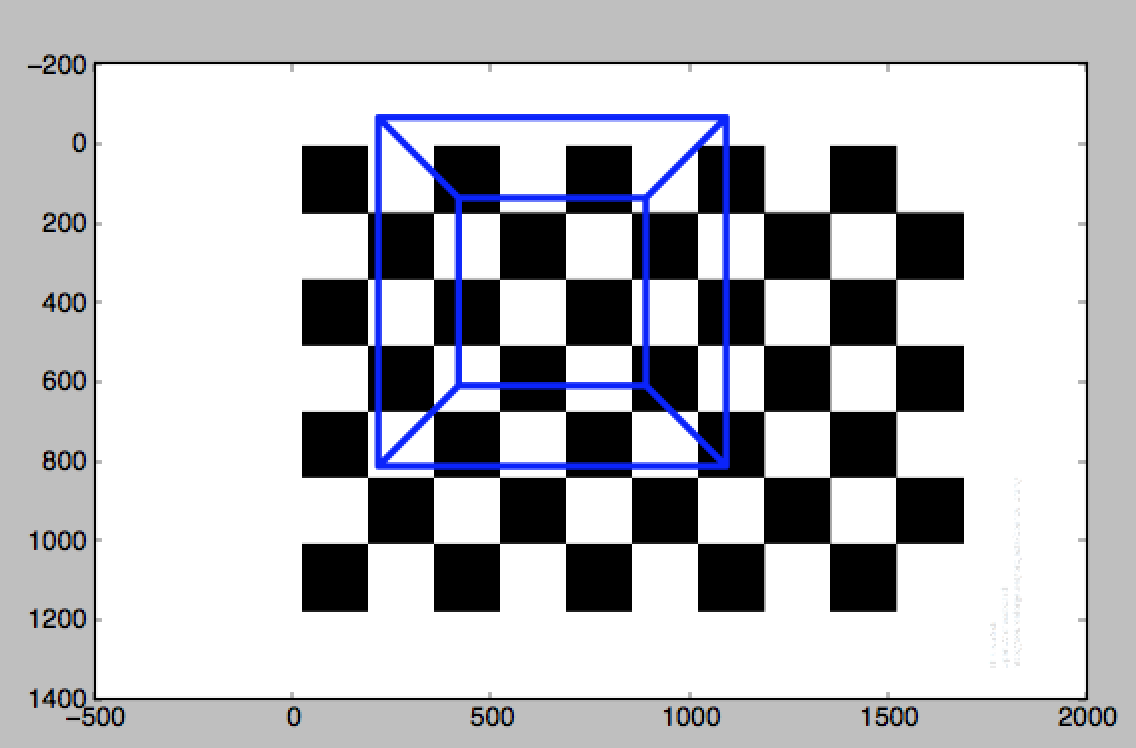
\includegraphics{pics/result0.png}
\caption{Our first projection onto the pattern image. The perspective projection effect is very visable on this image. Notice the translation of the pattern. This will affect the placement of the box on the rest of the images.}
\label{result0}
\end{figure}

\begin{figure}[H]
\center
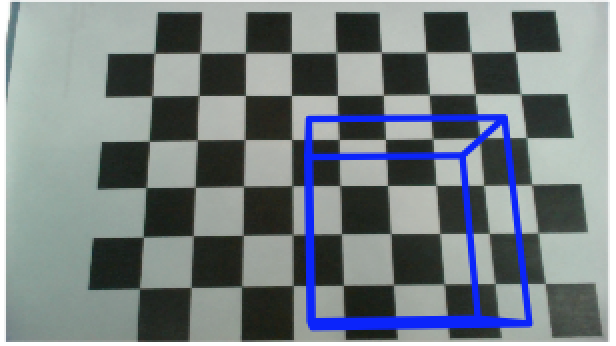
\includegraphics{pics/result1.png}
\caption{On this image the chessboard is only moved slightly away from the full frontal position. The position of the boc on the pattern doesn’t correspond to the position of the pattern image, but is consistent with the rest of the images.}
\label{result1}
\end{figure}

\begin{figure}[H]
\center
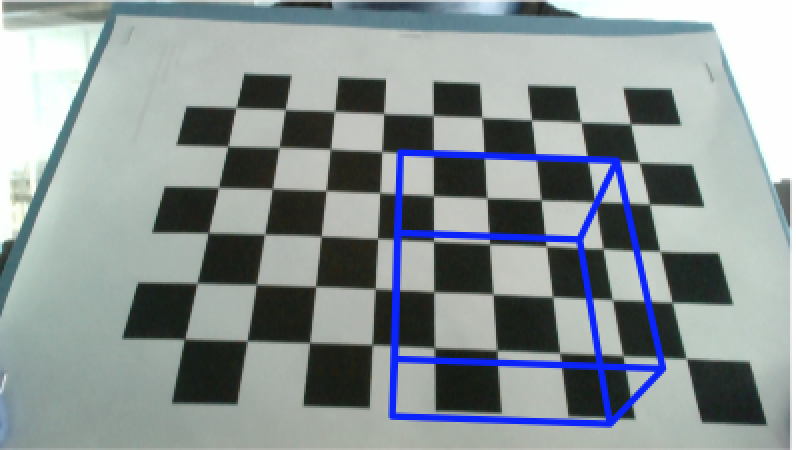
\includegraphics{pics/result2.png}
\caption{The 3d effect gets more pronounced as the chessboard is moved further away from the frontal position. The box doesn’t look completely even, but that is caused by the estimation of the z axis.}
\label{result2}
\end{figure}

\begin{figure}[H]
\center
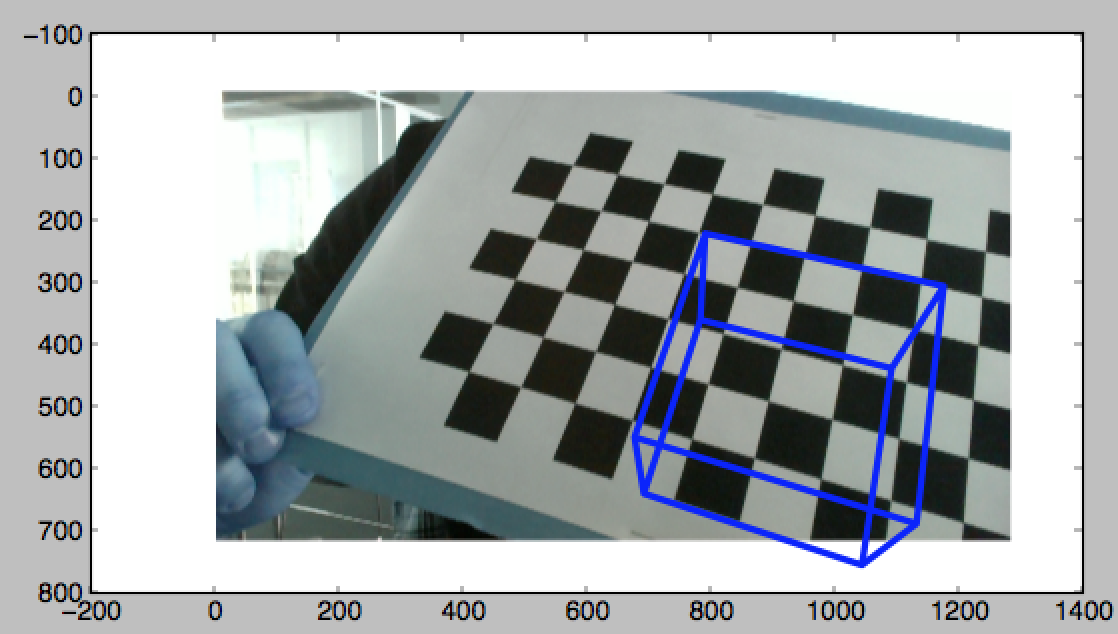
\includegraphics{pics/result3.png}
\caption{As we see here. The projection and plotting of the box, doesn’t care about image limits in this implementation. Gives a pretty nice effect though. (Best viewed with 3d glasses :-))}
\label{result3}
\end{figure}


\begin{figure}[H]
\center
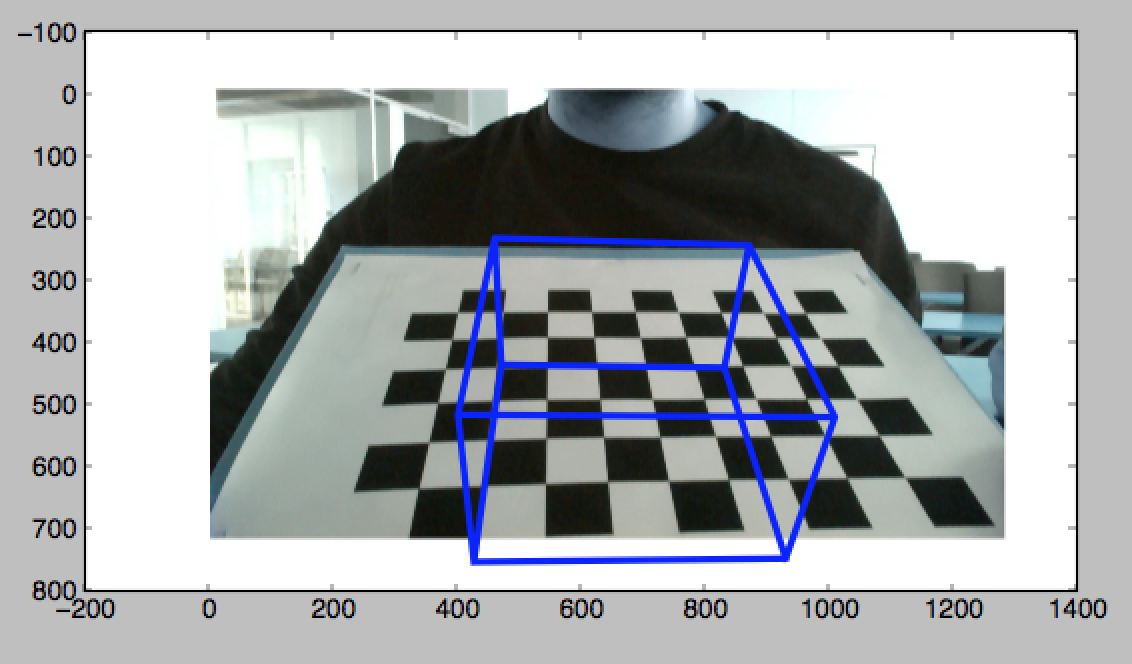
\includegraphics{pics/result4.png}
\caption{The augmentation effect works best when the surroundings are visible. Also note that the box looks a bit skewed/uneven but follows the chessboard pattern exactly because of the homography.}
\label{result4}
\end{figure}

\begin{figure}[H]
\center
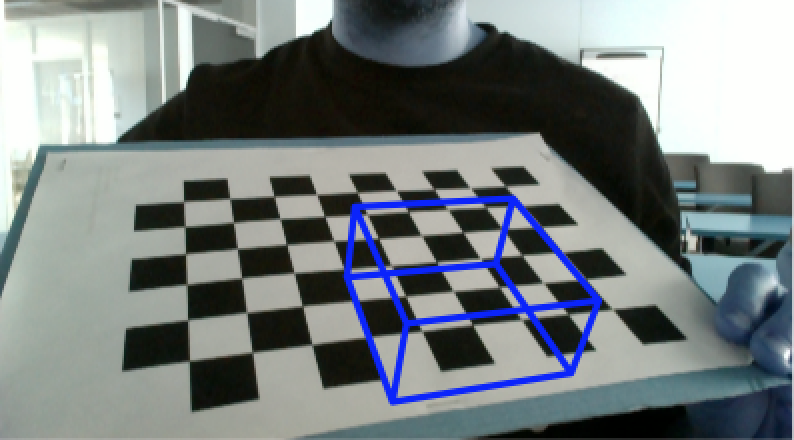
\includegraphics{pics/result5.png}
\caption{Last image. Lets just notice that it looks awesome. Next stop cool 3d models projected on family photos.}
\label{result5}
\end{figure}


\subsection{Taking it live}

As soon as the method for augmenting a box on a single frame is in place,
expanding to live view is a pretty easy task. 
In the old augmentation method we did a fair share of redundant
calculations. In order for the live augmentation to run smoothly, these had
to be moved out so they’ll only be done once.

Reading in the pattern image, converting it to greyscale and loading the
calibration-matrixes were moved out to global vars instead.

\begin{verbatim}
I1 = cv2.imread("pattern.png")
I1Gray = cv2.cvtColor(I1,cv2.COLOR_RGB2GRAY)
K, dist_coefs = calibrate.loadMatrixes()
\end{verbatim}

Calculating the corderns of the original pattern image, getting the box cords
and initialising the first camera instance also only needed to be done once.

\begin{verbatim}
I1Corners = getCornerCoords(I1Gray)
box = cube_points((0,0,0),0.3)
cam1 = Camera(hstack((K,dot(K,array([[0],[0],[-1]])) )) )
\end{verbatim}

Notice that these are only minor speed improvements, as each frame still has
some heavy calculations to be made:

\subsubsection{We still have to}
Find the chessboard corners on the supplied frame

\begin{verbatim}
I2Corners = getCornerCoords(I2Gray)
\end{verbatim}

Calculate a homography between the two chessboard 2d surfaces.

\begin{verbatim}
H = estimateHomography(I1Corners, I2Corners)
\end{verbatim}

Project the box cords onto the new surface.

\begin{verbatim}
box_cam2 = np.array(cam2.project(toHomogenious(box)))
\end{verbatim}

And then draw the box in the frame.
The end result could of course be improve further (as always), but for the scope
of this assignment we think the result is very acceptable, and undeniably cool
:-)
See. Aug.avi for the result video.



\section{Augmented reality}

What we want to achieve:
We want to calibrate a camera using cv2 implemented methods.
Grab images of the calibration chessboard.
Project a box onto the images, with a camera class calculated for each
image. 

\subsection{Camera Calibration}

Why do we calibrate?
We want to be aware of the factors within the camera, that may affect the
displaying of our  image.

\textbf{The focal length}, a measure for how much the used lens
centers/bends the light

\begin{figure}[!htbp]
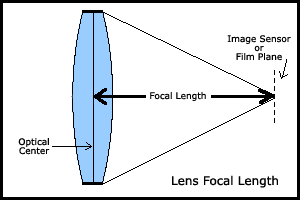
\includegraphics{pics/focal_length.png}
\caption{Focal length}
\label{fig:focal_length}
\end{figure}

\textbf{The image center} (according to the camera), this is not always just
positioned at precisely at half the height, half the width.
\textbf{Scaling factors}. Scaling can occur both horizontally and vertically. 
\textbf{Skew factors}.  Skewing may happen.
\textbf{Lens distortion}.  Cheap lenses may produce pin/cushion effects, and some
cameras may even add additional lenses to correct these issues.

All these factors needs to be taken into consideration when we wish to
calculate projections from the world coordinates to image coordinates. 

We calibrate the camera by using the cv2 implementation and a standard
calibration chessboard pattern. 


\subsection{Camera internal matrixes}

The camera consists of Intrinsic and extrinsic parameters,
K * [R | T]
The extrinsic parameters consists of a 3x3 rotation matrix (R )and a
translation vector (T). The translation vector expresses the origin of the world
coordinate system in camera coordinates. 
These transforms the coordinates from 3d world coordinates to 3d camera
coordinates. 

The intrinsic matrix (K) contains 5 parameters.

\begin{figure}[!htbp]
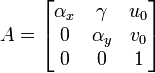
\includegraphics{pics/intristic_parameters.png}
\caption{Intrinsic/camera -matrix (here represented by "A")}
\label{fig:intrinsic_parameters}
\end{figure}

Alpha-X = focal length * scale factor(for x-coords), and 

Alpha-Y = focal length * scale factor(for y-coords). These converts real world
length (in mm) to pixel distance. 

$\gamma$  is the skew coefficient, and u0 v0 are the camera center.


\subsection{projecting and image using K* [I | O]}

\begin{figure}[H]
\centering
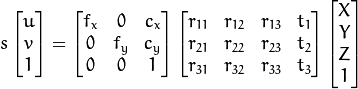
\includegraphics{pics/homogenious_projection.png}
\label{homogenious_projection}
\end{figure}

When we want to project 3d coordinates to the 2d image plane we multiply the
coord vector by K * [I | O] matrixes and converts the result to
homogeneous coords on the 2d image plane. Here (X,Y,Z) is the world
coordinate and (U,V) is the image coordinate. 
The column vectors [r1, r2, r3] of the “I” extrinsic matrix represent the
directions of the world-axes in camera coordinates.


\subsection{Theory of our implementation}

When we want to project a box onto different surfaces, we need to
calculate new camera parameters K * [I | O] each time we change
scene/angle. Some parameters can be reused. The intrinsic camera matrix “K”
doesn’t rely on anything from the scene and remains the same once calibrated. 

The first projection and the first camera.
The first camera initialized in our implementation uses the the fact that our
camera has been calibrated, and the projection plane is fully frontal and dead
center (in theory).
Therefore, no rotation and no translation in happening in the projection and
the [I | O] part of our camera class is equal to the identity matrix
(changes nothing when multiplied onto another matrix). 

The box cordinates are projected in the center of the image and viewed
directly from above.
As the projection is a perspective projection not a parallel projection, the
box appears realisticly to “pop” out from the surface. 

\begin{figure}[H]
\center
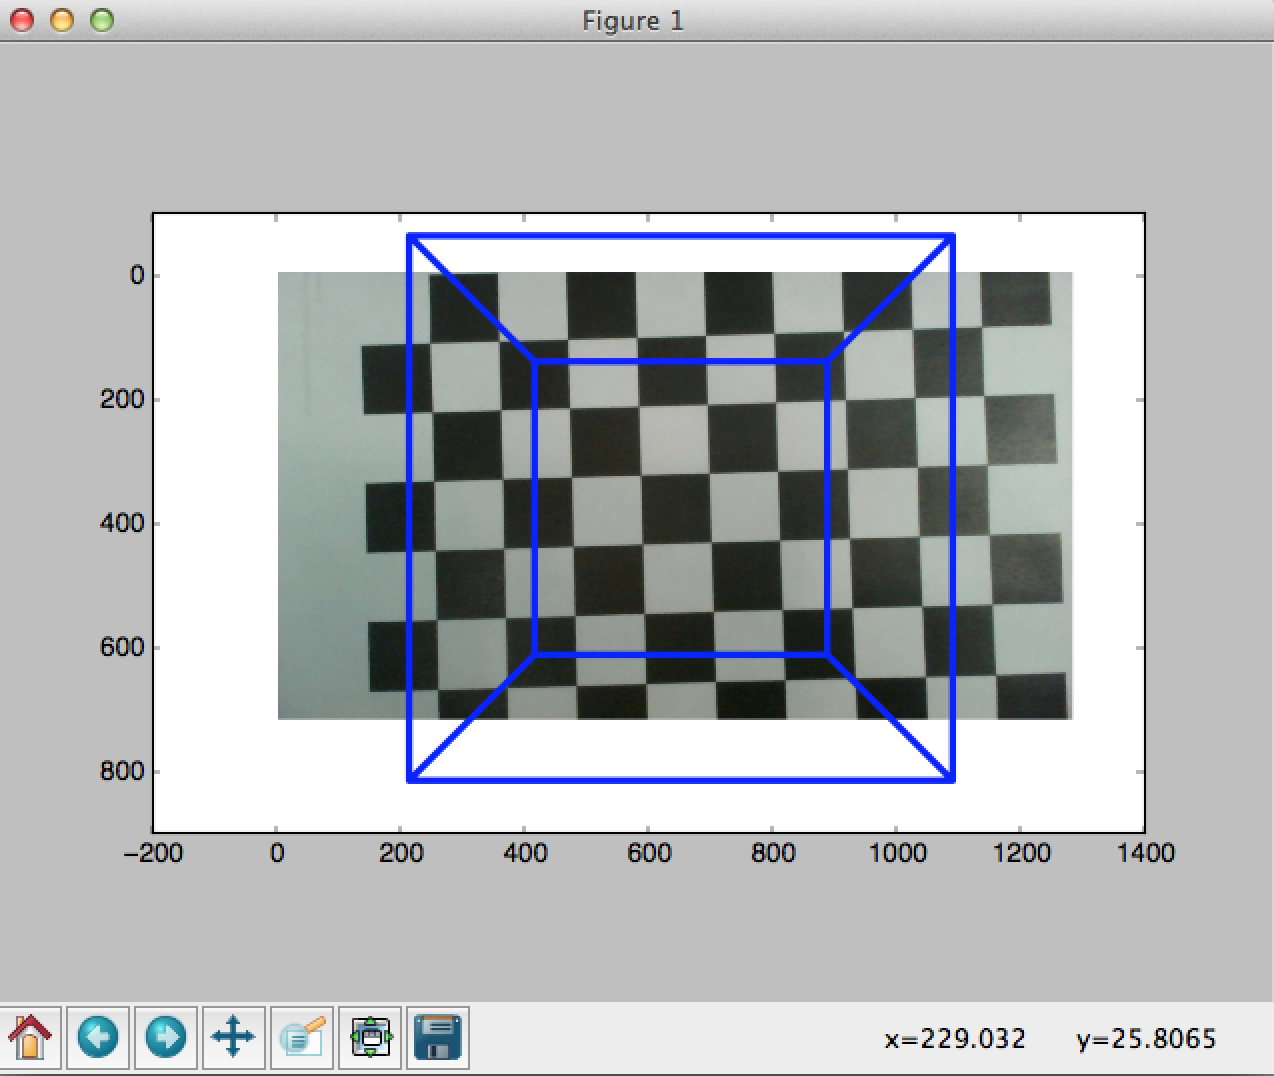
\includegraphics{pics/aug1}
\caption{The first projection onto a fully frontal surface.}
\label{aug1}
\end{figure}

When we want to project the box realistically onto the chessboard when the image
is no longer fully frontal, we calculate a new camera class.
This is done through the following steps:
1.We estimate a homography between the two chessboard surfaces, gaining a 2d
conversion between the two chessboards/scenes.
2.We multiply the existing camera with the homography as using the
homography is a perfectly valid way of projecting the 2D “X” and “Y” coords.
3.We estimate values for the “Z” axis by taking the cross product of the “X”
and “Y” axis-vectors. Thsi will always be orthogonal to both these
vectors, and therefore a good, but not precise estimation of the z-axis.


\begin{figure}[H]
\center
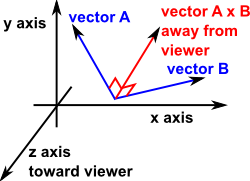
\includegraphics{pics/crossProduct.png}
\caption{Estimating the third axis from the existing two by taking the AxB crossproduct.}
\label{cross_product}
\end{figure}


\subsection{Our Code: (the important lines)}

\begin{verbatim}
//This line initializes the first camera, with K * [I | O] .

 cam1 = Camera(hstack((K,dot(K,array([[0],[0],[-1]])) )) )

//We estimate the homography “H” between the two chessboards by detecting 4 corners in each image.

H = estimateHomography(I1Corners, I2Corners)

//The homography is used on the existing (frontal) camera

  cam2 = Camera(dot(H,cam1.P))

//We isolate the [Rotation | translation] matrix by multiplying by inverse of “K” calibration matrix.

 A = dot(linalg.inv(K),cam2.P[:,:3]) 

//The intrinsic parameters are initialized. The X,Y axes are already valid after being multiplied by the homography matrix, and the third column vector is estimated with the cross product.

    A = array([A[:,0],A[:,1],np.cross(A[:,0],A[:,1],axis=0)]).T

// The calibration matrix is added again by multiplication, and the result is stored in the new camera.

    cam2.P[:,:3] = np.dot(K,A[0])

 //The box coordinates are projected onto the plane with the second camera

box_cam2 = np.array(cam2.project(toHomogenious(box)))
\end{verbatim}

Note: Concerning getting a better homography we found that using the
original pattern image “pattern.png” instead of our own frontal webcam
photo produced a better result. It proved hard to capture a frontal image
without any rotation or translation. At least with using the pattern image we
avoid rotations, but a translation is still present as the pattern is not
completely centered. 


\subsection{Augmentation, our results}

\begin{figure}[H]
\center
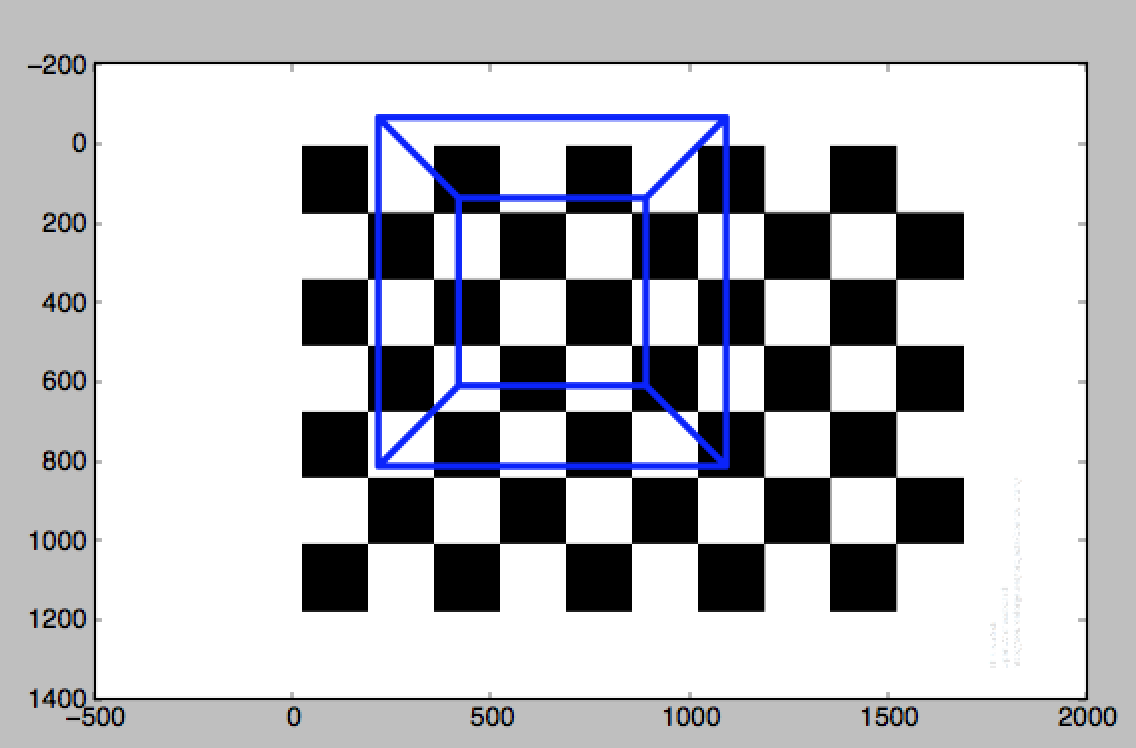
\includegraphics{pics/result0.png}
\caption{Our first projection onto the pattern image. The perspective projection effect is very visable on this image. Notice the translation of the pattern. This will affect the placement of the box on the rest of the images.}
\label{result0}
\end{figure}

\begin{figure}[H]
\center
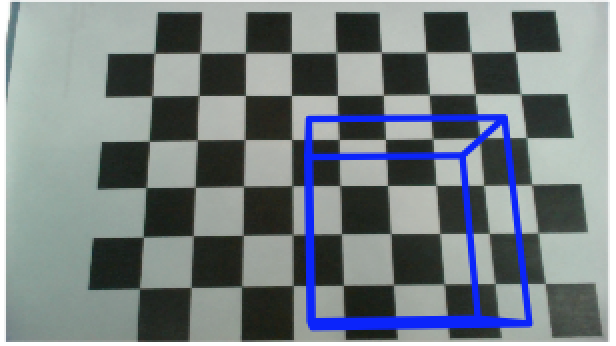
\includegraphics{pics/result1.png}
\caption{On this image the chessboard is only moved slightly away from the full frontal position. The position of the boc on the pattern doesn’t correspond to the position of the pattern image, but is consistent with the rest of the images.}
\label{result1}
\end{figure}

\begin{figure}[H]
\center
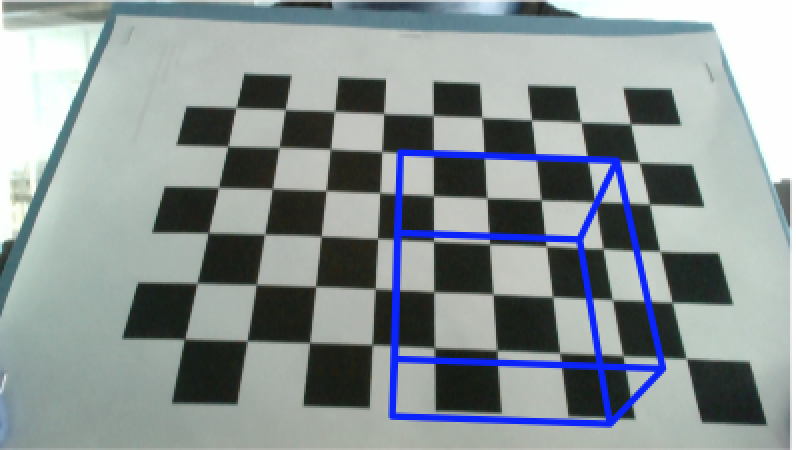
\includegraphics{pics/result2.png}
\caption{The 3d effect gets more pronounced as the chessboard is moved further away from the frontal position. The box doesn’t look completely even, but that is caused by the estimation of the z axis.}
\label{result2}
\end{figure}

\begin{figure}[H]
\center
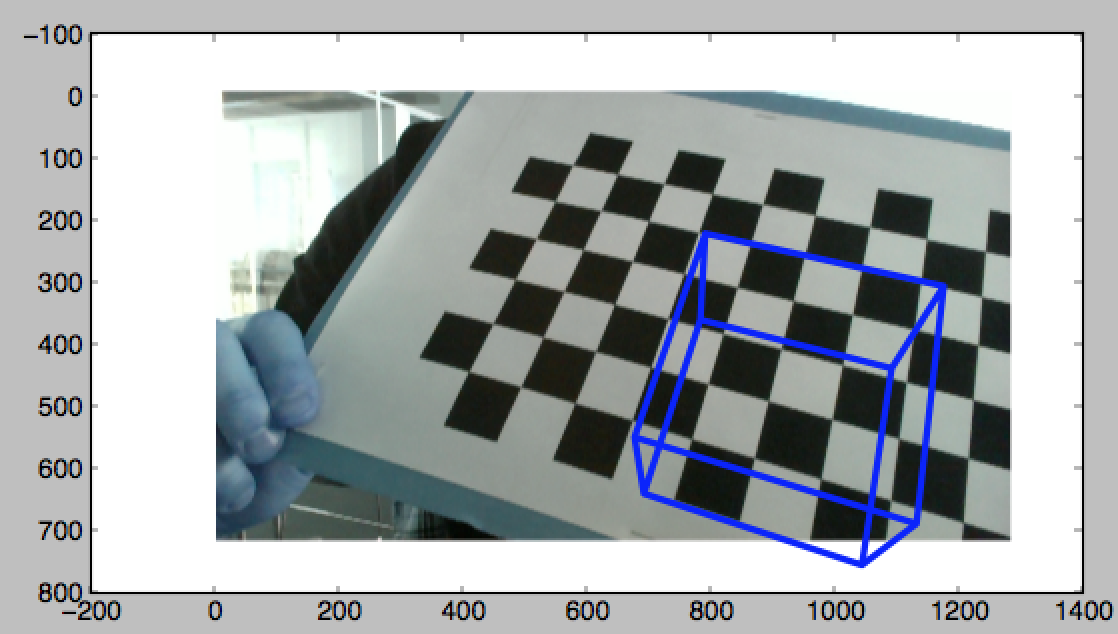
\includegraphics{pics/result3.png}
\caption{As we see here. The projection and plotting of the box, doesn’t care about image limits in this implementation. Gives a pretty nice effect though. (Best viewed with 3d glasses :-))}
\label{result3}
\end{figure}


\begin{figure}[H]
\center
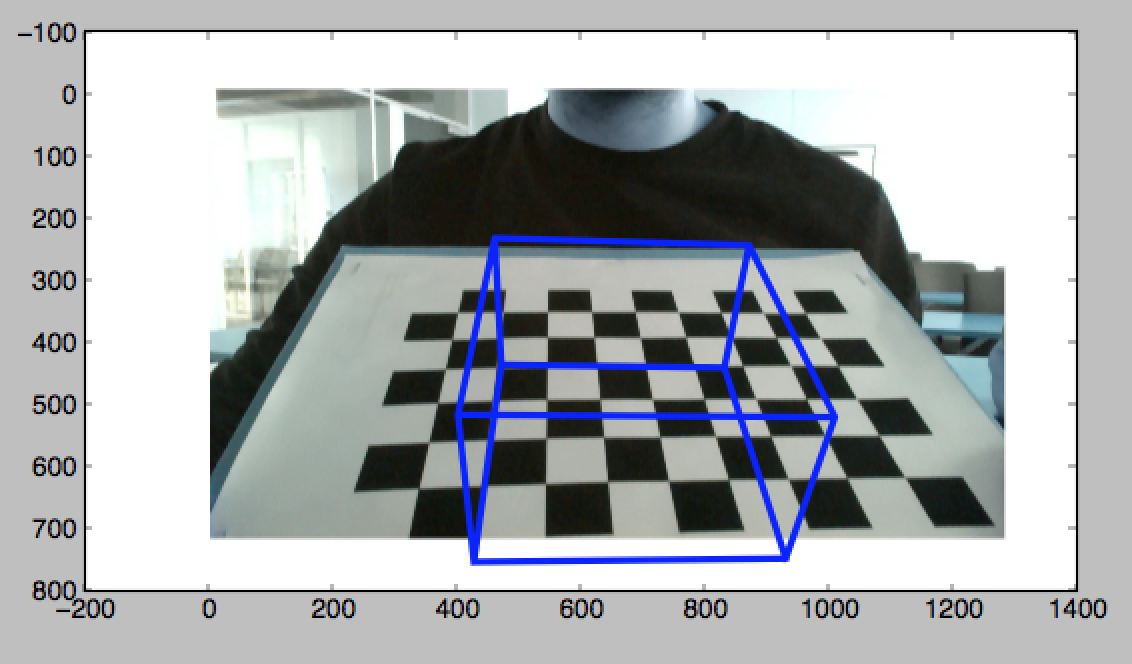
\includegraphics{pics/result4.png}
\caption{The augmentation effect works best when the surroundings are visible. Also note that the box looks a bit skewed/uneven but follows the chessboard pattern exactly because of the homography.}
\label{result4}
\end{figure}

\begin{figure}[H]
\center
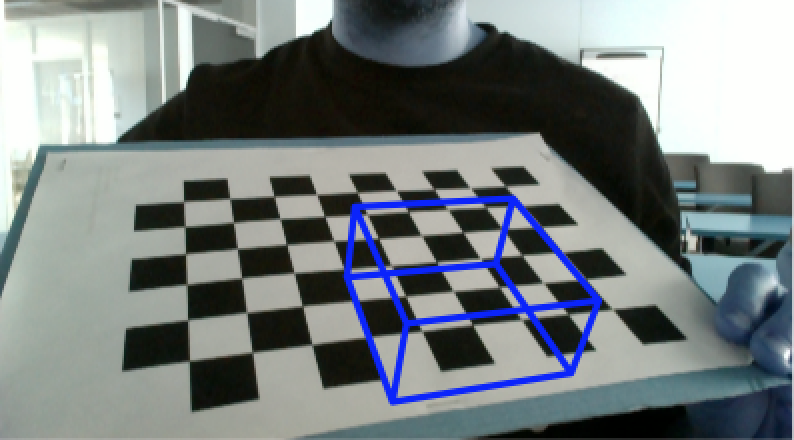
\includegraphics{pics/result5.png}
\caption{Last image. Lets just notice that it looks awesome. Next stop cool 3d models projected on family photos.}
\label{result5}
\end{figure}


\subsection{Taking it live}

As soon as the method for augmenting a box on a single frame is in place,
expanding to live view is a pretty easy task. 
In the old augmentation method we did a fair share of redundant
calculations. In order for the live augmentation to run smoothly, these had
to be moved out so they’ll only be done once.

Reading in the pattern image, converting it to greyscale and loading the
calibration-matrixes were moved out to global vars instead.

\begin{verbatim}
I1 = cv2.imread("pattern.png")
I1Gray = cv2.cvtColor(I1,cv2.COLOR_RGB2GRAY)
K, dist_coefs = calibrate.loadMatrixes()
\end{verbatim}

Calculating the corderns of the original pattern image, getting the box cords
and initialising the first camera instance also only needed to be done once.

\begin{verbatim}
I1Corners = getCornerCoords(I1Gray)
box = cube_points((0,0,0),0.3)
cam1 = Camera(hstack((K,dot(K,array([[0],[0],[-1]])) )) )
\end{verbatim}

Notice that these are only minor speed improvements, as each frame still has
some heavy calculations to be made:

\subsubsection{We still have to}
Find the chessboard corners on the supplied frame

\begin{verbatim}
I2Corners = getCornerCoords(I2Gray)
\end{verbatim}

Calculate a homography between the two chessboard 2d surfaces.

\begin{verbatim}
H = estimateHomography(I1Corners, I2Corners)
\end{verbatim}

Project the box cords onto the new surface.

\begin{verbatim}
box_cam2 = np.array(cam2.project(toHomogenious(box)))
\end{verbatim}

And then draw the box in the frame.
The end result could of course be improve further (as always), but for the scope
of this assignment we think the result is very acceptable, and undeniably cool
:-)
See. Aug.avi for the result video.



\section{Augmented reality}

What we want to achieve:
We want to calibrate a camera using cv2 implemented methods.
Grab images of the calibration chessboard.
Project a box onto the images, with a camera class calculated for each
image. 

\subsection{Camera Calibration}

Why do we calibrate?
We want to be aware of the factors within the camera, that may affect the
displaying of our  image.

\textbf{The focal length}, a measure for how much the used lens
centers/bends the light

\begin{figure}[!htbp]
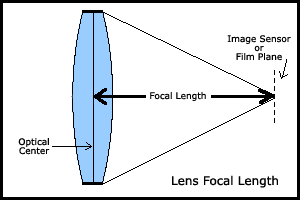
\includegraphics{pics/focal_length.png}
\caption{Focal length}
\label{fig:focal_length}
\end{figure}

\textbf{The image center} (according to the camera), this is not always just
positioned at precisely at half the height, half the width.
\textbf{Scaling factors}. Scaling can occur both horizontally and vertically. 
\textbf{Skew factors}.  Skewing may happen.
\textbf{Lens distortion}.  Cheap lenses may produce pin/cushion effects, and some
cameras may even add additional lenses to correct these issues.

All these factors needs to be taken into consideration when we wish to
calculate projections from the world coordinates to image coordinates. 

We calibrate the camera by using the cv2 implementation and a standard
calibration chessboard pattern. 


\subsection{Camera internal matrixes}

The camera consists of Intrinsic and extrinsic parameters,
K * [R | T]
The extrinsic parameters consists of a 3x3 rotation matrix (R )and a
translation vector (T). The translation vector expresses the origin of the world
coordinate system in camera coordinates. 
These transforms the coordinates from 3d world coordinates to 3d camera
coordinates. 

The intrinsic matrix (K) contains 5 parameters.

\begin{figure}[!htbp]
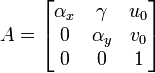
\includegraphics{pics/intristic_parameters.png}
\caption{Intrinsic/camera -matrix (here represented by "A")}
\label{fig:intrinsic_parameters}
\end{figure}

Alpha-X = focal length * scale factor(for x-coords), and 

Alpha-Y = focal length * scale factor(for y-coords). These converts real world
length (in mm) to pixel distance. 

$\gamma$  is the skew coefficient, and u0 v0 are the camera center.


\subsection{projecting and image using K* [I | O]}

\begin{figure}[H]
\centering
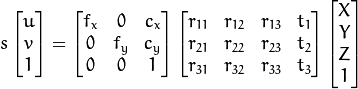
\includegraphics{pics/homogenious_projection.png}
\label{homogenious_projection}
\end{figure}

When we want to project 3d coordinates to the 2d image plane we multiply the
coord vector by K * [I | O] matrixes and converts the result to
homogeneous coords on the 2d image plane. Here (X,Y,Z) is the world
coordinate and (U,V) is the image coordinate. 
The column vectors [r1, r2, r3] of the “I” extrinsic matrix represent the
directions of the world-axes in camera coordinates.


\subsection{Theory of our implementation}

When we want to project a box onto different surfaces, we need to
calculate new camera parameters K * [I | O] each time we change
scene/angle. Some parameters can be reused. The intrinsic camera matrix “K”
doesn’t rely on anything from the scene and remains the same once calibrated. 

The first projection and the first camera.
The first camera initialized in our implementation uses the the fact that our
camera has been calibrated, and the projection plane is fully frontal and dead
center (in theory).
Therefore, no rotation and no translation in happening in the projection and
the [I | O] part of our camera class is equal to the identity matrix
(changes nothing when multiplied onto another matrix). 

The box cordinates are projected in the center of the image and viewed
directly from above.
As the projection is a perspective projection not a parallel projection, the
box appears realisticly to “pop” out from the surface. 

\begin{figure}[H]
\center
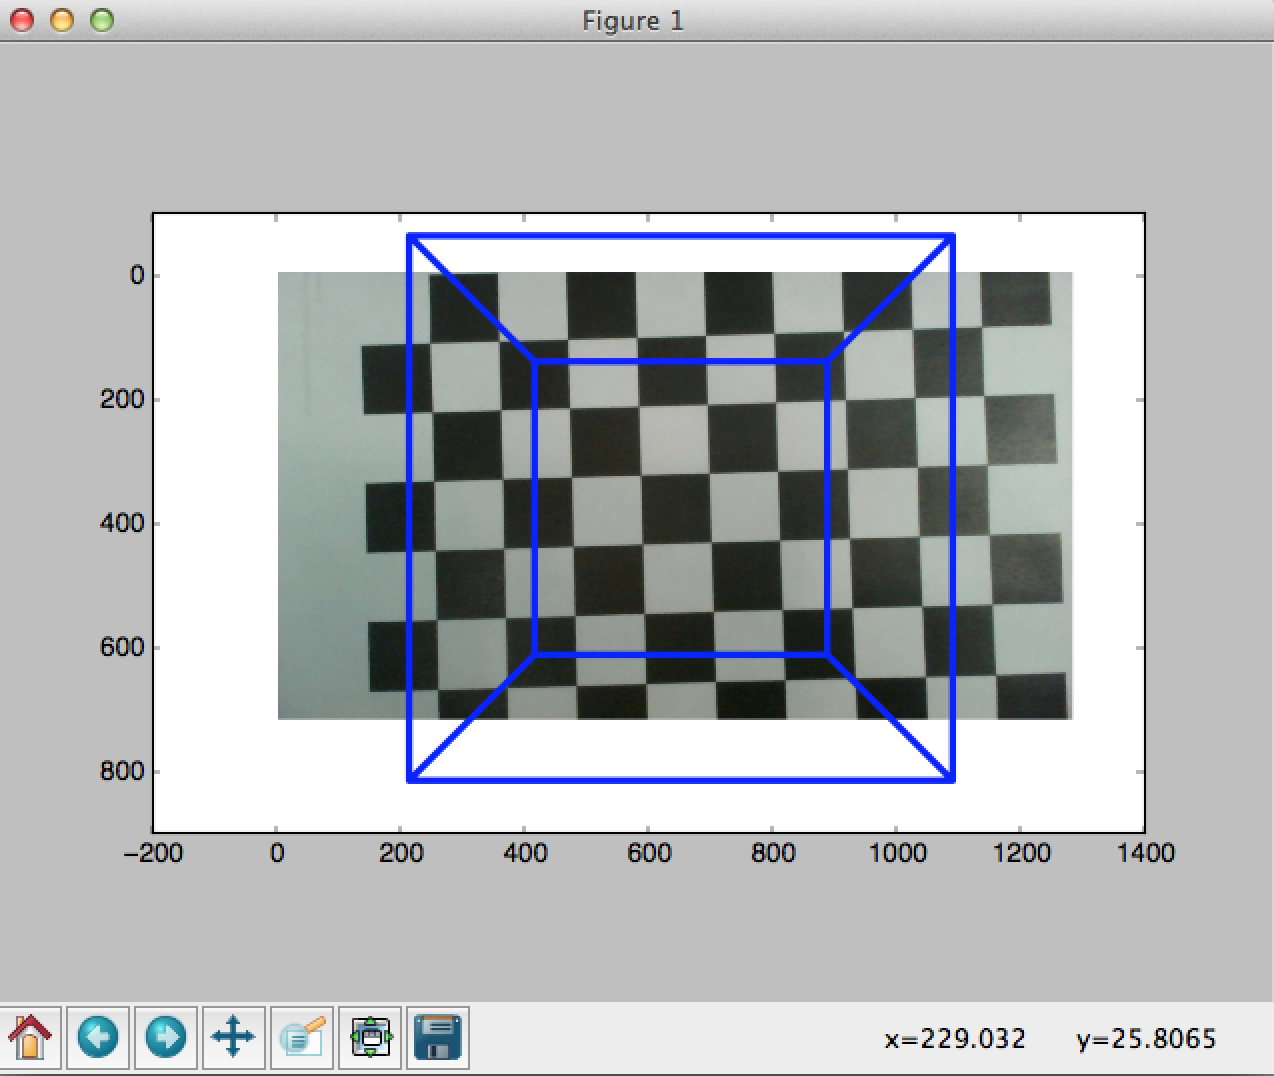
\includegraphics{pics/aug1}
\caption{The first projection onto a fully frontal surface.}
\label{aug1}
\end{figure}

When we want to project the box realistically onto the chessboard when the image
is no longer fully frontal, we calculate a new camera class.
This is done through the following steps:
1.We estimate a homography between the two chessboard surfaces, gaining a 2d
conversion between the two chessboards/scenes.
2.We multiply the existing camera with the homography as using the
homography is a perfectly valid way of projecting the 2D “X” and “Y” coords.
3.We estimate values for the “Z” axis by taking the cross product of the “X”
and “Y” axis-vectors. Thsi will always be orthogonal to both these
vectors, and therefore a good, but not precise estimation of the z-axis.


\begin{figure}[H]
\center
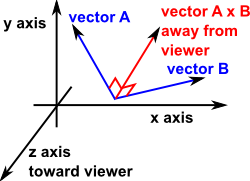
\includegraphics{pics/crossProduct.png}
\caption{Estimating the third axis from the existing two by taking the AxB crossproduct.}
\label{cross_product}
\end{figure}


\subsection{Our Code: (the important lines)}

\begin{verbatim}
//This line initializes the first camera, with K * [I | O] .

 cam1 = Camera(hstack((K,dot(K,array([[0],[0],[-1]])) )) )

//We estimate the homography “H” between the two chessboards by detecting 4 corners in each image.

H = estimateHomography(I1Corners, I2Corners)

//The homography is used on the existing (frontal) camera

  cam2 = Camera(dot(H,cam1.P))

//We isolate the [Rotation | translation] matrix by multiplying by inverse of “K” calibration matrix.

 A = dot(linalg.inv(K),cam2.P[:,:3]) 

//The intrinsic parameters are initialized. The X,Y axes are already valid after being multiplied by the homography matrix, and the third column vector is estimated with the cross product.

    A = array([A[:,0],A[:,1],np.cross(A[:,0],A[:,1],axis=0)]).T

// The calibration matrix is added again by multiplication, and the result is stored in the new camera.

    cam2.P[:,:3] = np.dot(K,A[0])

 //The box coordinates are projected onto the plane with the second camera

box_cam2 = np.array(cam2.project(toHomogenious(box)))
\end{verbatim}

Note: Concerning getting a better homography we found that using the
original pattern image “pattern.png” instead of our own frontal webcam
photo produced a better result. It proved hard to capture a frontal image
without any rotation or translation. At least with using the pattern image we
avoid rotations, but a translation is still present as the pattern is not
completely centered. 


\subsection{Augmentation, our results}

\begin{figure}[H]
\center
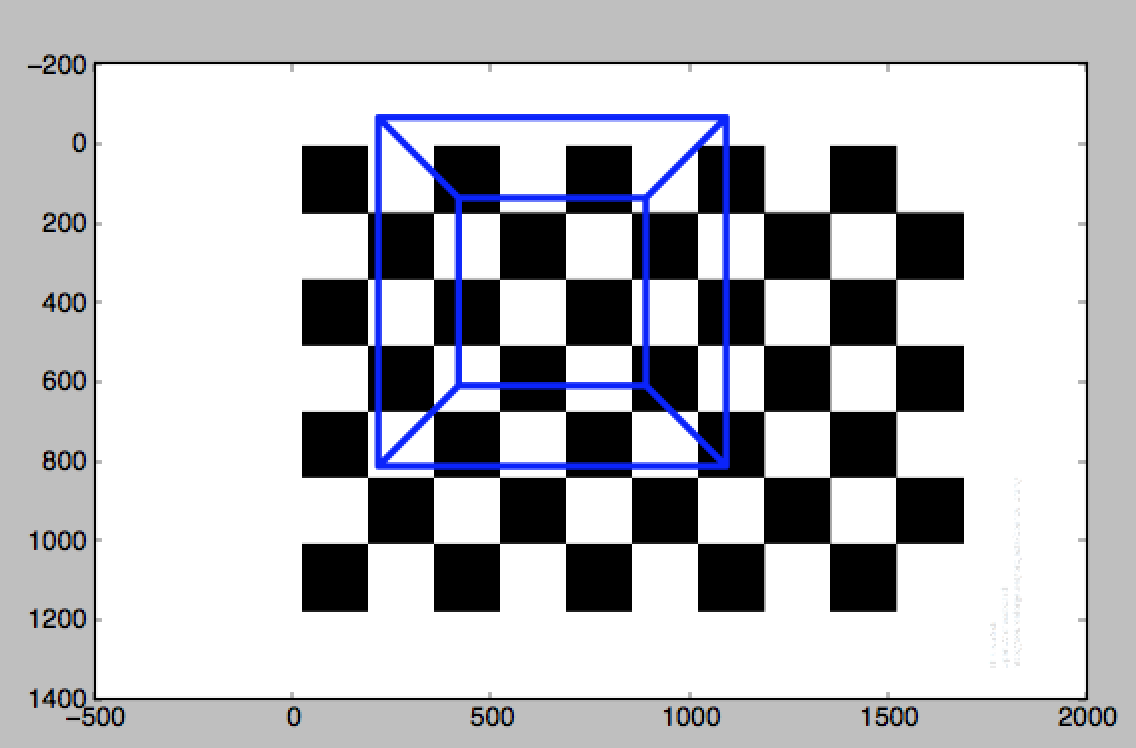
\includegraphics{pics/result0.png}
\caption{Our first projection onto the pattern image. The perspective projection effect is very visable on this image. Notice the translation of the pattern. This will affect the placement of the box on the rest of the images.}
\label{result0}
\end{figure}

\begin{figure}[H]
\center
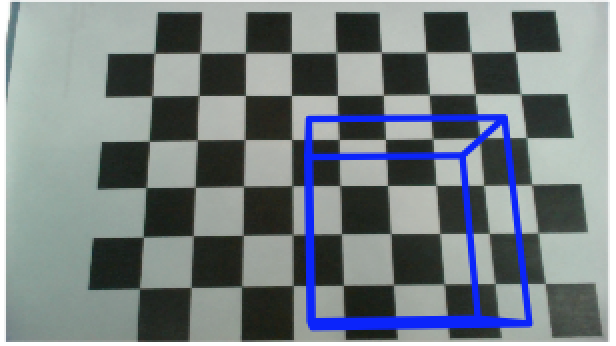
\includegraphics{pics/result1.png}
\caption{On this image the chessboard is only moved slightly away from the full frontal position. The position of the boc on the pattern doesn’t correspond to the position of the pattern image, but is consistent with the rest of the images.}
\label{result1}
\end{figure}

\begin{figure}[H]
\center
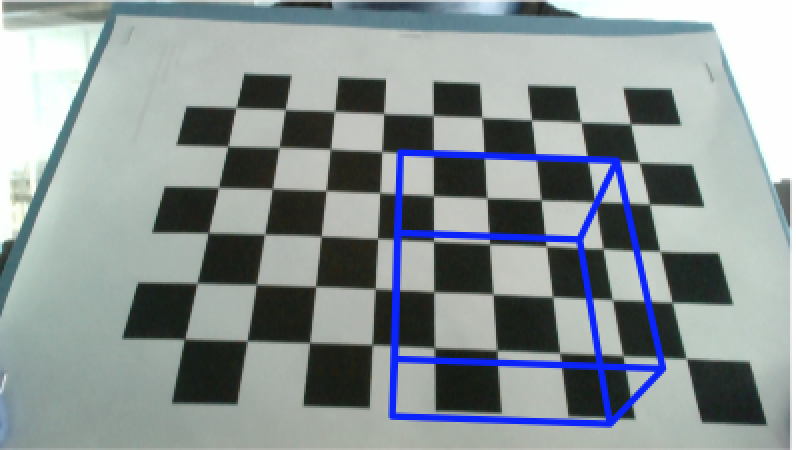
\includegraphics{pics/result2.png}
\caption{The 3d effect gets more pronounced as the chessboard is moved further away from the frontal position. The box doesn’t look completely even, but that is caused by the estimation of the z axis.}
\label{result2}
\end{figure}

\begin{figure}[H]
\center
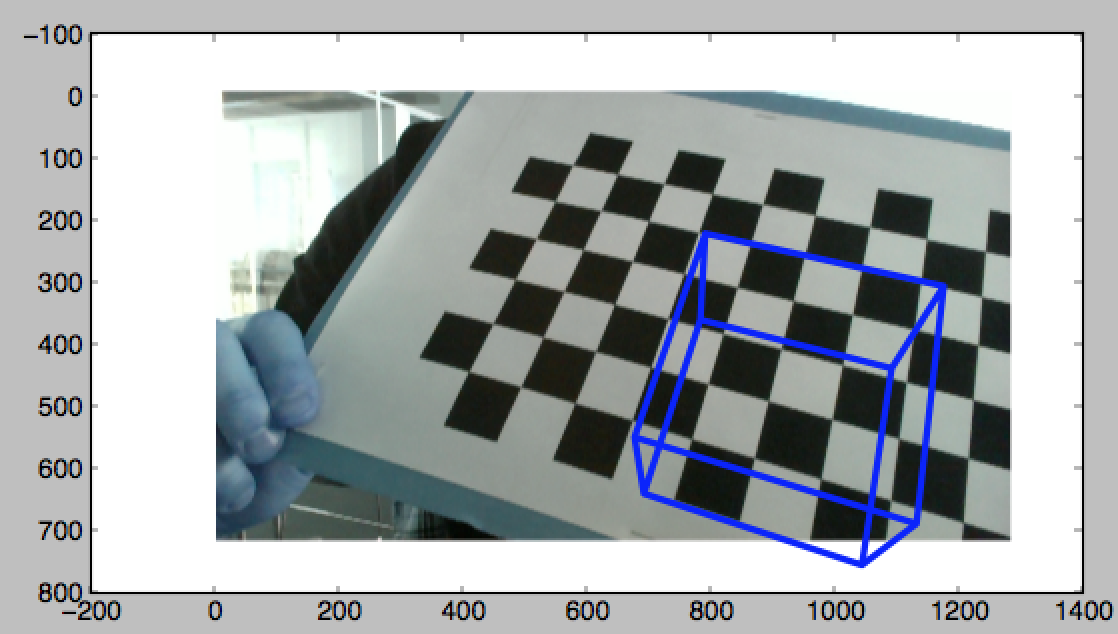
\includegraphics{pics/result3.png}
\caption{As we see here. The projection and plotting of the box, doesn’t care about image limits in this implementation. Gives a pretty nice effect though. (Best viewed with 3d glasses :-))}
\label{result3}
\end{figure}


\begin{figure}[H]
\center
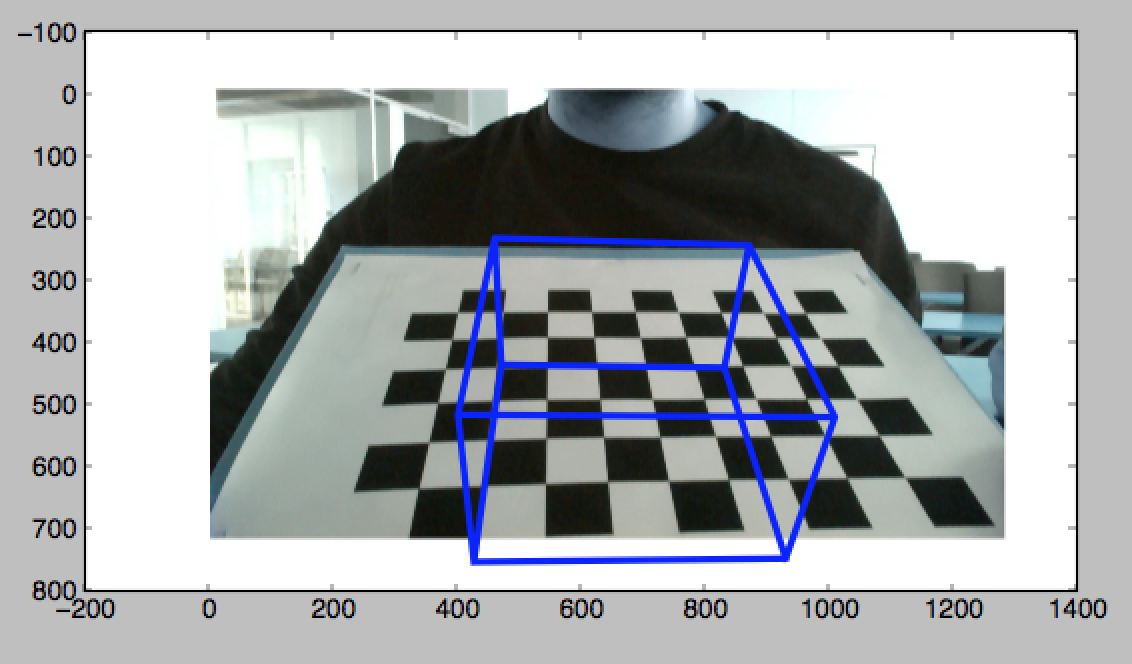
\includegraphics{pics/result4.png}
\caption{The augmentation effect works best when the surroundings are visible. Also note that the box looks a bit skewed/uneven but follows the chessboard pattern exactly because of the homography.}
\label{result4}
\end{figure}

\begin{figure}[H]
\center
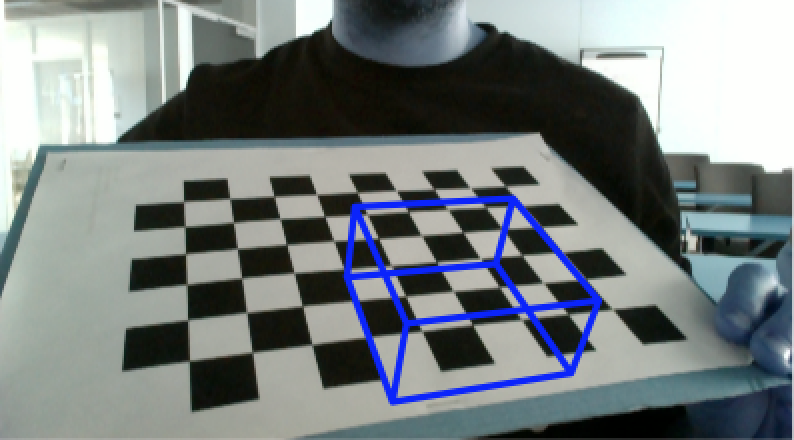
\includegraphics{pics/result5.png}
\caption{Last image. Lets just notice that it looks awesome. Next stop cool 3d models projected on family photos.}
\label{result5}
\end{figure}


\subsection{Taking it live}

As soon as the method for augmenting a box on a single frame is in place,
expanding to live view is a pretty easy task. 
In the old augmentation method we did a fair share of redundant
calculations. In order for the live augmentation to run smoothly, these had
to be moved out so they’ll only be done once.

Reading in the pattern image, converting it to greyscale and loading the
calibration-matrixes were moved out to global vars instead.

\begin{verbatim}
I1 = cv2.imread("pattern.png")
I1Gray = cv2.cvtColor(I1,cv2.COLOR_RGB2GRAY)
K, dist_coefs = calibrate.loadMatrixes()
\end{verbatim}

Calculating the corderns of the original pattern image, getting the box cords
and initialising the first camera instance also only needed to be done once.

\begin{verbatim}
I1Corners = getCornerCoords(I1Gray)
box = cube_points((0,0,0),0.3)
cam1 = Camera(hstack((K,dot(K,array([[0],[0],[-1]])) )) )
\end{verbatim}

Notice that these are only minor speed improvements, as each frame still has
some heavy calculations to be made:

\subsubsection{We still have to}
Find the chessboard corners on the supplied frame

\begin{verbatim}
I2Corners = getCornerCoords(I2Gray)
\end{verbatim}

Calculate a homography between the two chessboard 2d surfaces.

\begin{verbatim}
H = estimateHomography(I1Corners, I2Corners)
\end{verbatim}

Project the box cords onto the new surface.

\begin{verbatim}
box_cam2 = np.array(cam2.project(toHomogenious(box)))
\end{verbatim}

And then draw the box in the frame.
The end result could of course be improve further (as always), but for the scope
of this assignment we think the result is very acceptable, and undeniably cool
:-)
See. Aug.avi for the result video.



\section{Aaaand then whatever Unge Roed makes :)}

\end{document}
